\section{Material and Methods}

\subsection{Bibliometric Approach}
Bibliometric analysis studies bibliographic data quantitatively, through performance analysis and science mapping \parencite{donthu2021,zupic2015}. This study uses four techniques that answer different questions. Citation analysis identifies the most influential documents, co-citation analysis reveals the foundations of the field, bibliographic coupling shows its current research streams, and co-word analysis maps its concepts.

\subsection{Search Strings}
Records were retrieved from OpenAlex through its public interface on 28 October 2026. OpenAlex is an open index of scholarly works, authors, sources, and institutions \parencite{priem2022}. The search covered titles and abstracts, was restricted to the document type ``article'', and covered the publication years 2023 to 2026, of which 2026 is incomplete. OpenAlex was chosen because it is open and its queries can be repeated. Most bibliometric guidance assumes Scopus or Web of Science \parencite{donthu2021}, and the choice between these databases is discussed by \textcite{zhu2020}, \textcite{mongeon2016}, and \textcite{echchakoui2020}. The consequences of using OpenAlex instead are discussed in the Discussion section.

Table~\ref{tab:search} lists the search strings. Each row holds synonyms joined with OR, and the rows are combined into three blocks, one for each stream. Block A (LLM agents in business settings) combines rows 1, 3, and 4 with AND. Block B (LLMs in the browser or on the device) combines rows 2 and 5. Block C (LLMs for inventory) combines rows 2, 6, and 7 and excludes records that match row 8.

\begin{table}[htbp]
\centering
\normalsize
\caption{Search string in OpenAlex database}
\label{tab:search}
\begin{tabularx}{\textwidth}{cYY}
\hline
\textbf{No} & \textbf{Keywords} & \textbf{Justification} \\ \hline
1 & ``large language model'' OR LLM OR LLMs & To identify literature related to LLMs (block A) \\
2 & ``large language model'' OR LLM OR LLMs OR ``small language model'' OR SLM & To identify literature related to language models, including small ones (blocks B and C) \\
3 & ``multi-agent'' OR multiagent OR agentic OR ``LLM agent'' OR ``LLM agents'' & To identify literature related to multi-agent and agentic LLM systems \\
4 & ``inventory management'' OR ``inventory control'' OR ``supply chain management'' OR SME OR SMEs OR ``small business'' OR ``small businesses'' OR retail OR MSME OR ``business process'' & To restrict block A to business and operational settings \\
5 & WebLLM OR WebGPU OR ``in-browser'' OR ``browser-based'' OR ``on-device'' OR ``edge device'' OR ``edge devices'' & To identify literature related to models that run in the browser, on the device, or at the edge \\
6 & inventory OR stock & To identify literature related to inventory and stock \\
7 & retail OR SME OR SMEs OR ``small business'' OR ``small businesses'' OR MSME OR warehouse OR ``supply chain management'' OR procurement OR ``demand forecasting'' OR ``sales forecasting'' OR replenishment OR ``point of sale'' OR e-commerce & To place inventory in a business context \\
8 & NOT (``stock market'' OR ``stock price'' OR ``stock prices'' OR ``stock exchange'' OR ``stock trading'' OR ``stock returns'') & To exclude studies about share prices, where ``stock'' has a different meaning \\ \hline
\end{tabularx}
\par\vspace{2pt}Source: Authors' construction.
\end{table}

\subsection{Screening and Final Dataset}
The three blocks returned 149, 584, and 87 records, 820 in total, which formed 801 unique records (Table~\ref{tab:flow}). Sixteen records shared a normalised title with another record; in each case the version with a journal source, reference data, and a DOI was kept. A further 77 records hosted on Zenodo were excluded, because Zenodo is a repository without a guaranteed peer-review process. The remaining 708 records were screened on title and abstract.

Screening was assisted by language models in two passes. In the first pass, eight Claude Haiku instances judged about 89 records each as relevant, not relevant, or uncertain. A record counted as relevant when a language model and at least one of the three topics were a main or important part of the work. The pass produced 430 relevant, 150 not relevant, and 128 uncertain records. In the second pass, three Claude Sonnet instances reassessed the 128 uncertain records using longer abstracts and reported a confidence level. They resolved 55 records as relevant and 72 as not relevant and left one uncertain. Generative AI was therefore used in this study for screening, and also for data processing scripts and text drafting (see Section~3.5 and the Acknowledgements). The model reported low confidence for 97 of the 128 second-pass decisions. The first author therefore judged 20 low-confidence records without seeing the model labels. The first author rated all 20 as relevant, whereas the model had rated 8 as relevant and 12 as not relevant. Agreement was 8 of 20 (40\%), and Cohen's kappa was 0 because the first author used a single category. The disagreement ran in one direction only: every record that the model excluded was rated relevant by the first author. The sample covers only low-confidence decisions and does not estimate the accuracy of the full screening, but it shows that the exclusions made in the second pass are open to dispute. All 72 second-pass exclusions were therefore assessed a third time by a larger model, Claude Opus 5.5, which read the full abstracts against the written criteria and recorded a reason for each record. It rated 4 records as relevant and 68 as not relevant. The 68 include the 12 records that the first author had rated as relevant in the sample; in them the language model or the topic is a minor part of the work, for example a cloud model that serves edge devices or an agent framework outside business operations. The difference between the sample ratings and the third assessment thus lies in how strictly a ``main or important part'' is read. The first author chose to apply the criteria as written and adopted the third assessment, so the final dataset contains 489 records.

\begin{table}[htbp]
\centering
\normalsize
\caption{Record flow}
\label{tab:flow}
\begin{tabularx}{\textwidth}{YcY}
\hline
\textbf{Step} & \textbf{Records} & \textbf{Note} \\ \hline
Retrieved (blocks A, B, C) & 820 & 149, 584, and 87 records \\
Unique records & 801 & 19 records matched more than one block \\
After removing duplicate titles & 785 & 16 removed \\
After excluding Zenodo & 708 & 77 removed \\
Included after screening & 489 & 218 not relevant, 1 unresolved \\ \hline
\end{tabularx}
\par\vspace{2pt}Source: Authors' analysis of OpenAlex data.
\end{table}

\subsection{Analysis}
Performance analysis counted publications per year, source, institution, country (from author affiliations), and author, together with citations. Authors, sources, and institutions were counted by OpenAlex identifiers rather than names. Science mapping used three techniques \parencite{donthu2021,zupic2015}.

Co-word analysis used the keywords that OpenAlex assigns to each record. Synonymous forms were merged (for example ``LLM'' and ``large language models''), and ``large language model'' and ``artificial intelligence'' were dropped because they occur in nearly every record. Keywords with at least eight occurrences were kept, which gave 69 keywords.

Bibliographic coupling and co-citation rely on reference lists. OpenAlex held reference data for 259 of the 489 records. Crossref data, matched through DOIs, raised the total to 282 records (57.7\%). Two records were treated as linked when they shared at least two references. A rule set by the supervising authors asks for three to five clusters per map, each with at least six items. For bibliographic coupling this was met by keeping only articles cited at least three times and removing clusters of fewer than six articles after clustering. For co-citation, references cited by at least three records in the dataset were kept. Ten items were removed as data artefacts. Some were proceedings volumes, which are not single works. Three were references whose OpenAlex titles do not fit the articles that cite them: one is cited by 22 edge-LLM articles although its title concerns intelligent tutoring systems, and two are cited by 9 and 7 edge-LLM articles although their titles concern AI consciousness and behavioural safety. These look like linking errors in OpenAlex, but this was not verified.

The thresholds of three citations and eight occurrences were chosen so that each map contains a readable number of items (347 references and 69 keywords). Figure~\ref{fig:ambang} shows how many items remain at other thresholds. The curves fall steadily and have no sharp break, so the choice is a judgement, and the robustness checks below vary the co-word threshold.

\begin{figure}[htbp]
\centering
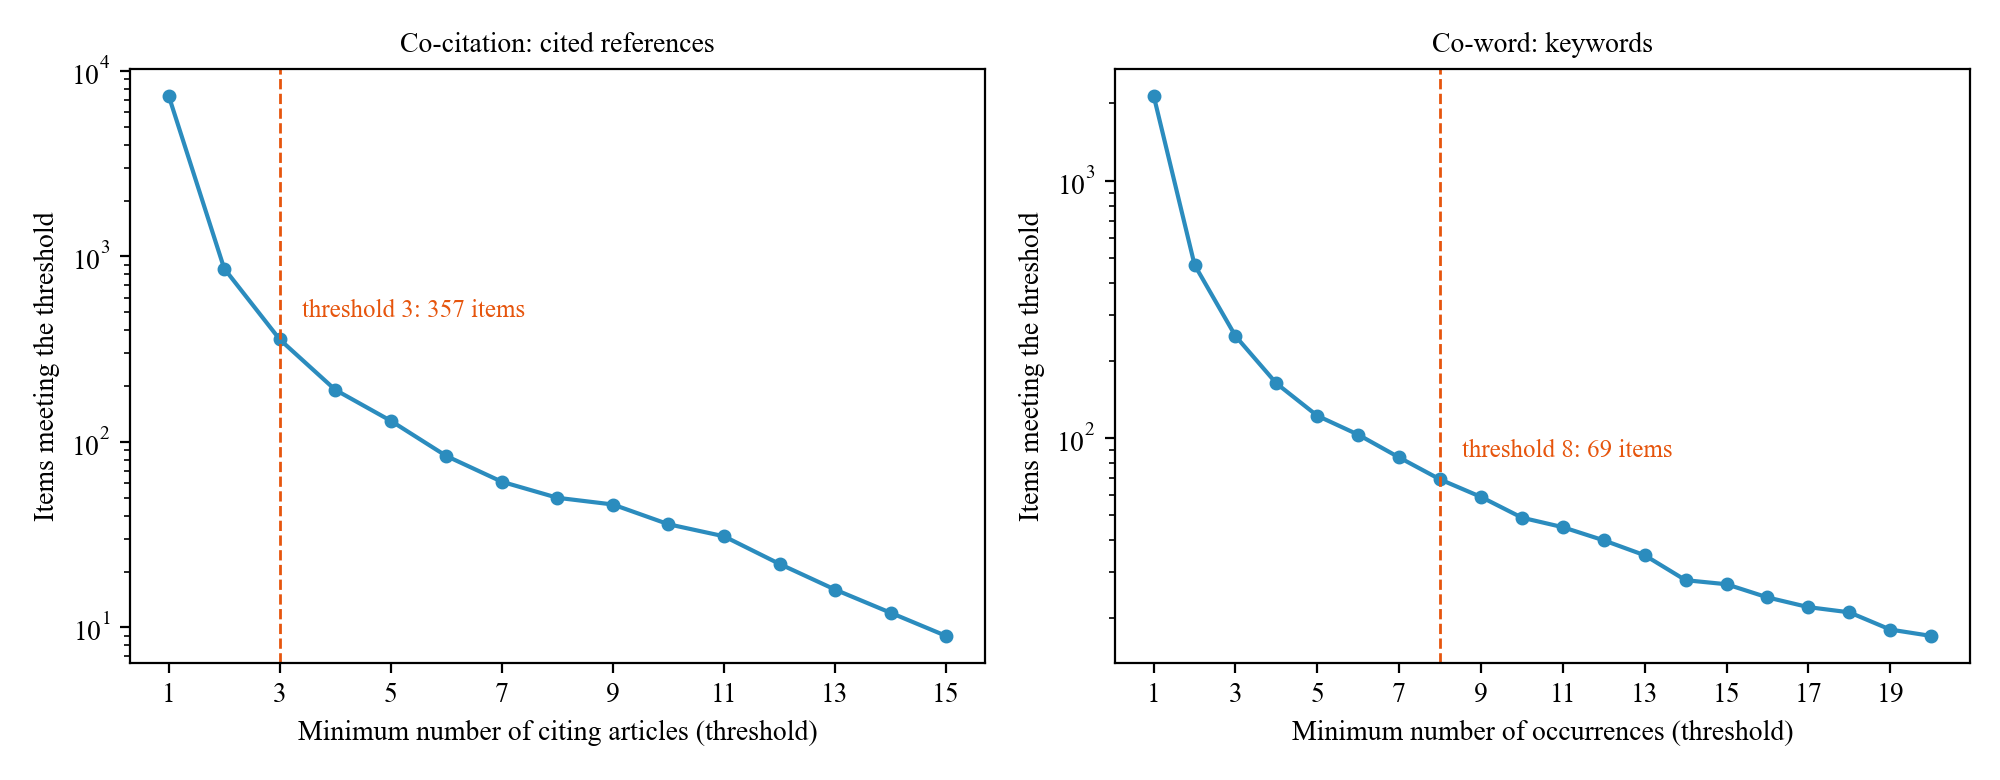
\includegraphics[width=\textwidth]{figures/fig_ambang.png}
\par\vspace{2pt}Source: Authors' analysis of OpenAlex data.
\caption{Number of items meeting each minimum threshold (left: references by number of citing articles, counted before the ten artefacts were removed; right: keywords by number of occurrences)}
\label{fig:ambang}
\end{figure}

Clusters were found with the Louvain algorithm \parencite{blondel2008}, computed in Python (networkx, fixed random seed) and displayed in VOSviewer 1.6.21 \parencite{vaneck2010} through its map and network file formats. The cluster membership shown in the figures is therefore the one computed in Python. Robustness was tested in several ways. The co-word clustering was repeated with minimum occurrences of 5, 8, and 12, with 20 random seeds, and with a greedy modularity algorithm. The coupling clustering (without the citation threshold) and the co-citation clustering were repeated with 20 seeds and the greedy algorithm. Five variations of the search strings were also run. Cluster names were chosen by the first author from proposals made with language-model assistance, after reading the members of each cluster: keywords and representative articles for co-word, reference titles for co-citation, and article titles for coupling. The dataset is above the minimum of about 200 papers that \textcite{rogers2020} suggest for stable average citation indicators; their study concerns institutional citation impact rather than science mapping, so the figure is used only as a rough lower bound. The record flow follows the PRISMA statement \parencite{page2021}.

\subsection{Tools, Roles, and Dates}
Table~\ref{tab:tools} states which tool was used at each step, for what, when, and by whom. Dates are in 2026. Every step was run by the first author through Claude Code (Anthropic), which executed the scripts and, where marked, delegated the screening to separate model instances. The first author set the research questions, the search blocks, the screening criteria, and the thresholds, and made every decision about inclusion rules, clustering, and wording. Scopus, Web of Science, Zotero, and Biblioshiny were not used for any reported result. R 4.6.1 with the bibliometrix package was installed but produced no result in this article; the thematic map follows the centrality and density definitions of Biblioshiny but was computed in Python.

\begin{table}[htbp]
\centering
\footnotesize
\caption{Tools, tasks, dates, and actors}
\label{tab:tools}
\begin{tabularx}{\textwidth}{p{0.13\textwidth}YYp{0.08\textwidth}p{0.14\textwidth}}
\hline
\textbf{Step} & \textbf{Tool and version} & \textbf{Task and method} & \textbf{Date} & \textbf{Actor} \\ \hline
Search and download & OpenAlex REST API (api.openalex.org), cursor paging, free API key & Title and abstract search of blocks A, B, and C; type ``article''; 2023 to 2026; 820 records retrieved (801 unique) & 28 Oct & Author; script run by Claude Code \\
Cleaning & Python 3.11.7, pandas 2.2.2 & Removed 16 duplicate titles and 77 Zenodo records; 708 records left & 28 Oct & First author's rules; script by Claude Code \\
Screening, first pass & Claude Haiku 5.5 (\texttt{claude-haiku-5-5}), 8 instances of about 89 records each, run as subagents in Claude Code & Judged title and abstract as relevant, not relevant, or uncertain & 28 Oct & Model; criteria set by the first author \\
Screening, second pass & Claude Sonnet 5.5 (\texttt{claude-sonnet-5-5}), 3 instances & Re-judged the 128 uncertain records with longer abstracts and a confidence level & 28 Oct & Model; criteria set by the first author \\
Human check & The first author's own reading of title and abstract & Blind rating of 20 low-confidence records (model labels hidden) & 29 Oct & Author \\
Screening, third pass & Claude Opus 5.5 (\texttt{claude-opus-5-5}) in Claude Code & Re-judged the 72 second-pass exclusions and the 14 low-confidence inclusions of the wider-search check with full abstracts and a reason per record & 29 Oct & Model; criteria set and result adopted by the first author \\
Reference completion & Crossref REST API (public pool), OpenAlex DOI matching & Added reference lists for 23 records whose OpenAlex reference data were empty & 29 Oct & Author; script run by Claude Code \\
Performance analysis & Python, pandas 2.2.2; OpenAlex identifiers & Counts of publications and citations by year, source, institution, country, and author; h-index & 28 to 29 Oct & Author; script run by Claude Code \\
Science mapping & Python, networkx 3.6.1 (Louvain algorithm, fixed seed; greedy modularity as check), matplotlib 3.8.3 & Co-word, co-citation, and bibliographic coupling networks; thresholds and robustness runs & 28 to 29 Oct & First author's thresholds; script run by Claude Code \\
Map display & VOSviewer 1.6.21 on Java 1.8.0\_481 & Opened the map and network files and exported the images from the command line & 28 to 29 Oct & Author; Claude Code started the export \\
Wider-search check & OpenAlex REST API; Claude Sonnet 5.5, 2 instances & Screened 127 added records (blocks A and C); kept as a sensitivity check only & 29 Oct & First author's decision; model screening \\
Reference check & Reference lookup tool over OpenAlex and arXiv & Checked that cited works exist (title, first author, DOI) & 28 to 29 Oct & Claude Code; author to read each work \\
Writing and typesetting & Claude Code (Claude Sonnet 5.5 and Claude Opus 5.5) for drafting; XeLaTeX (MiKTeX 25.12, XeTeX 3.141592653-2.6-0.999997), biblatex 3.21, Biber 2.21 & Drafted the text and tables from script output; APA 7 references & 28 to 29 Oct & Claude Code drafted; the authors review and edit \\ \hline
\end{tabularx}
\par\vspace{2pt}Source: Authors' record of the workflow.
\end{table}

Table~\ref{tab:data} describes the final dataset of 489 articles.

\begin{table}[htbp]
\centering
\footnotesize
\caption{Characteristics of the final dataset (489 articles)}
\label{tab:data}
\begin{tabularx}{\textwidth}{YY}
\hline
\textbf{Item} & \textbf{Value} \\ \hline
Articles by year & 2023: 4; 2024: 37; 2025: 153; 2026: 295 (partial) \\
Articles by search block & B: 351; A: 83; C: 41; A and C: 14; none matched A, B, and C together \\
Screening route & 430 relevant in the first pass; 55 in the second pass; 4 in the third pass \\
Metadata present & Title 489 (100\%); abstract 448 (91.6\%); DOI 462 (94.5\%); OpenAlex keywords 488 (99.8\%); source 483 (98.8\%); country 372 (76.1\%) \\
Reference lists & OpenAlex 259 (53.0\%); with Crossref 282 (57.7\%) \\
Citations (OpenAlex counts) & Total 2{,}910; mean 5.95 per article; median 0; 291 articles (59.5\%) uncited; h-index 24 \\
Journals flagged for checking & 23 articles; flagged by publisher-name patterns, not by a quality judgement \\ \hline
\end{tabularx}
\par\vspace{2pt}Source: Authors' analysis of OpenAlex data.
\end{table}
